\section{Data Analysis}

\begin{frame}{Data Analysis}{}
	\begin{itemize}
		\item {Simulation Bunches}
		\item {Data Handler Scripts}
		\item {Empirical Results}
	\end{itemize}
		
		\begin{equation}
			score(c,s) = \frac{\sum\limits^{N(c,s)}{i=0} pmatch(creq_{i},s)}{gap_{AVG}(c,s) + 1}
		\end{equation}

\end{frame}

\subsection{Simulation Bunches}
	

\subsection{Data Handler Scripts}
	\begin{frame}{Data Handler Scripts}
		%TODO pictures 
	\end{frame}

	\begin{frame}{Netbuilder}
		Genereates an XML file that describes the network
			
		\begin{figure}[H]
			\centering
			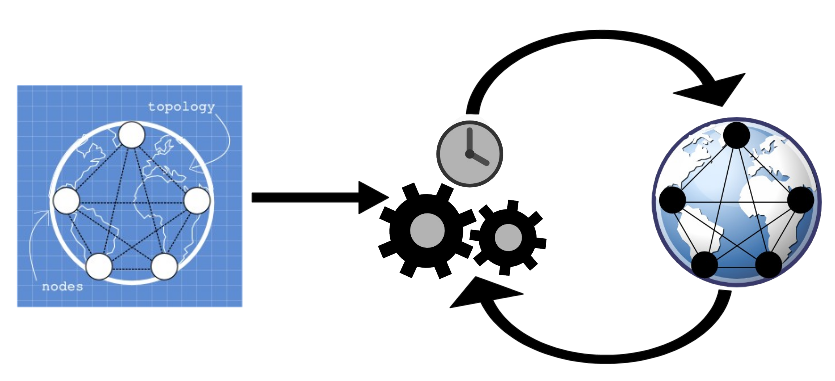
\includegraphics[scale=0.35]{design1.png}
		\end{figure}
	\end{frame}

	\begin{frame}{Netbuilder}
		Allow the network configuration through:
		\begin{itemize}
			
			\item The number of TOR exit nodes in the simulation.
			\item The number of TOR 4authorities\footnote{A 4 Authority node is simply the
			database that keep track of the state of the TOR network and the list
			of the TOR relays/exit-nodes} nodes in the simulation.
			\item The number of clients (simpletcp) of the simulation.
			\item The number of servers (simpletcp) of the simulation.
			\item The percentage of clients tracked by an autosys plug-in.
			\item The percentage of servers tracked by an autosys plug-in.
			\item The density of the network-requests.
		\end{itemize}
	\end{frame}	

	\begin{frame}{Netbuilder}
		The connection densities are the sleep time thresholds between each client connection request:
			
		\begin{itemize}
			\item Slow: 800 (mean) - 2000 (mean) milliseconds 			
			\item Average: 80 (mean)  - 1000 (mean) millisecons
			\item Fast: 20 (mean) - 100 (mean) milliseconds
		\end{itemize}
	\end{frame}			
	

	\begin{frame}{Launcher}
		\begin{center}
			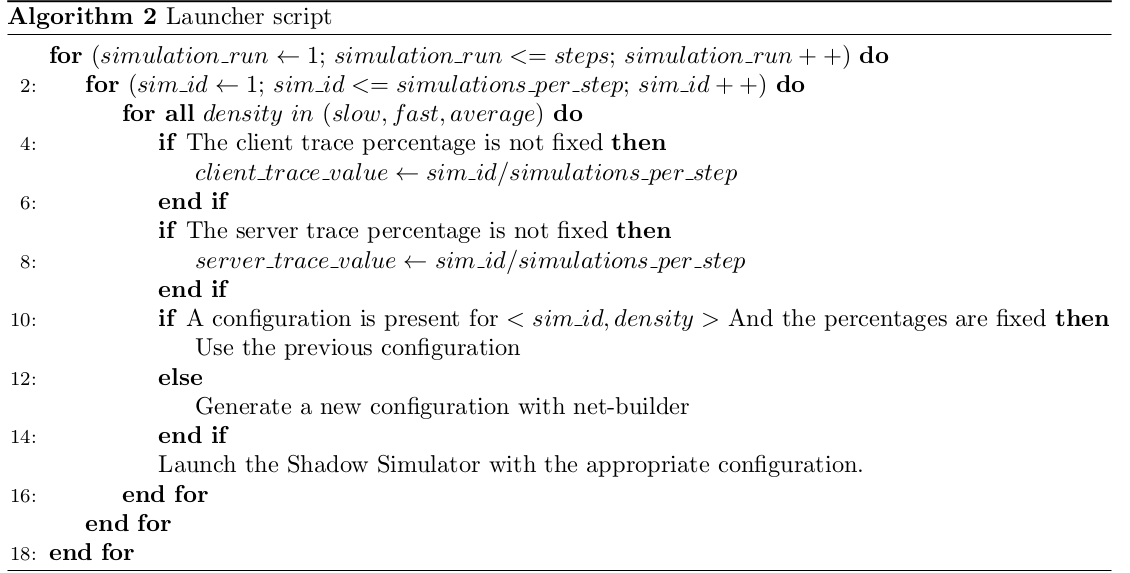
\includegraphics[scale=0.30]{algolauncher.png}
		\end{center}				

	\end{frame}

	\begin{frame}{Analyzer}

	\end{frame}



\subsection{Empirical Results}
